\documentclass{beamer}

\usepackage{../macros}

\title{Array}

\begin{document}

\frame{
  \titlepage
}

\begin{frame}[fragile]{Array}
  
  \begin{block}{}
    \begin{itemize}
      \item A collection of items stored at contiguous memory locations
      \item Data structure to store multiple items of the same type
    \end{itemize}
  \end{block}
  
  \begin{block}{}
    \centering
    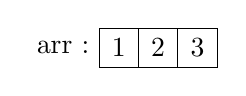
\begin{tikzpicture}[scale = 0.5]
      \draw (0, 0) rectangle (3, 1) 
        (1, 0) -- (1, 1)
        (2, 0) -- (2, 1);
      \draw (0.5, 0.5) node {1};
      \draw (1.5, 0.5) node {2};
      \draw (2.5, 0.5) node {3};
      \draw (0, 0.5) node[left] {arr :};
    \end{tikzpicture}
  \end{block}
  
  \begin{minipage}{0.48\textwidth}
    \begin{code}{In Python}
      \begin{lstlisting}[style=codePy]
arr = [1, 2, 3]
      \end{lstlisting}
    \end{code}
    
    \begin{code}{In R}
      \begin{lstlisting}[style=codeR]
arr <- c(1, 2, 3)
      \end{lstlisting}
    \end{code}
  
%    \begin{code}{In Shell}
%      \begin{lstlisting}[style=codeS]
%arr = (1 2 3)
%      \end{lstlisting}
%    \end{code}
  \end{minipage}\hfill
  \begin{minipage}{0.48\textwidth}
    \begin{code}{In C}
      \begin{lstlisting}[style=codeC]
int[] arr = {1, 2, 3};
      \end{lstlisting}
    \end{code}
  
    \begin{code}{In Java}
      \begin{lstlisting}[style=codeJ]
int[] arr = {1, 2, 3};
      \end{lstlisting}
    \end{code}
  \end{minipage}
\end{frame}

\begin{frame}{Exercise 1: Making Book}
  \begin{block}{Statement}
    Given two numbers $A$ and $B$, count the number of occurrences of each digit in the range between $A$ and $B$ included
  \end{block}
  
  \pause
  \begin{block}{Representation}
    \centering
    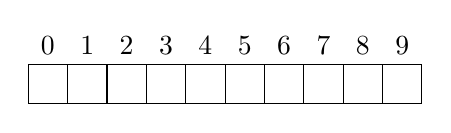
\begin{tikzpicture}[scale = 0.5]
      \draw (0, 0) rectangle (10, 1);
      \foreach \x in {1, 2, ..., 9}
        \draw (\x, 0) -- (\x, 1);
      \foreach \x in {0, 1, ..., 9}
        \draw ({\x + 0.5}, 1) node[above] {\x};
    \end{tikzpicture}
  \end{block}
  
  \pause
  \begin{example}
    \begin{columns}[T]
      \begin{column}{0.17\linewidth}
        \emphv{Input:}\\
        10 15\\
%        15 104\\
%        220 202\\
%        0
      \end{column}
      \begin{column}{0.79\linewidth}
        \emphv{Output:}\\
        Case 1: 0:1 1:7 2:1 3:1 4:1 5:1 6:0 7:0 8:0 9:0\\
%        Case 2: 0:14 1:19 2:19 3:19 4:19 5:19 6:19 7:19 8:19 9:19\\
%        Case 3: 0:10 1:11 2:22 3:2 4:2 5:2 6:2 7:2 8:2 9:2
      \end{column}
    \end{columns}
  \end{example}
\end{frame}

\begin{frame}{Exercise 1: Making Book}
  Quels problèmes on peut rencontrer ?
  $a > b, a = b$ ?
  taille de la solution ? entier ? plus ?
\end{frame}

\begin{frame}{Exercise 1: Making Book}
  Exemples de solutions
    - force brute
    - en réfléchissant un peu
\end{frame}

\begin{frame}{Exercise 2: It's a Murder}
  \begin{block}{Statement}
    Given an array of integers, for each number sum the previous strictly smaller number 
  \end{block}
  
  \pause
  \begin{block}{Representation}
    \centering
    \begin{tikzpicture}[scale = 0.5]
      \draw (0, 0) rectangle (5, 1);
      \foreach \x in {1, 2, ..., 5}
        \draw (\x, 0) -- (\x, 1);
      \draw (0.5, 0.5) node {\only<4, 5>\emphr{1}};
      \draw (1.5, 0.5) node {\only<6, 7>\emphr{5}};
      \draw (2.5, 0.5) node {\only<8, 9>\emphr{3}};
      \draw (3.5, 0.5) node {6};
      \draw (4.5, 0.5) node {4};
      
      \uncover<3->{
      \draw (0, -1.5) rectangle (5, -0.5);
      \foreach \x in {1, 2, ..., 5}
        \draw (\x, -1.5) -- (\x, -0.5);
      }
      
      \uncover<5->{\draw (0.5, -1) node {0};}
      \only<6, 7>{\draw[rose, thick] (0, 0) rectangle (1, 1);}
      \uncover<7->{\draw (1.5, -1) node {1};}
      \only<8, 9>{\draw[rose, thick] (0, 0) rectangle (2, 1);}
      \uncover<9->{\draw (2.5, -1) node {1};}
      \uncover<10->{
      \draw (3.5, -1) node {9};
      \draw (4.5, -1) node {4};
      }
    \end{tikzpicture}
  \end{block}
  
  \uncover<11->{
  \begin{example}
    \begin{columns}[T]
      \begin{column}{0.17\linewidth}
        \emphv{Input:}\\
        1\\5\\1 5 3 6 4%\\7\\1 3 5 2 6 7 4
      \end{column}
      \begin{column}{0.79\linewidth}
        \emphv{Output:}\\
        15%\\40
      \end{column}
    \end{columns}
  \end{example}}

  
  
\end{frame}

\end{document}
